\documentclass[aspectratio=169,xcolor=table]{beamer}
%aspcetratio >> 1610 169 149 54 43 32
%The themes:
%\usetheme[style=classic]{mharvellous}
%\usetheme[style=dark]{mharvellous}
%\usetheme[style=mracula]{mharvellous}
\usetheme[style=default]{mharvellous}
%*--------------------------------------------------
%\usepackage{helvet}
%*--------------------------------------------------
\usepackage{bibunits}  
%\setbeamertemplate{bibliography item}{[\theenumiv]}
\setbeamertemplate{bibliography item}{\insertbiblabel}
\defaultbibliography{bibliography}
%\defaultbibliographystyle{IEEEtran}
%\defaultbibliographystyle{amsalpha}
\defaultbibliographystyle{abntex2-alf}
%\bibliography{bibliography}
%\usepackage[backend=biber,style=alphabetic,citestyle=authoryear]{biblatex}
% \addbibresource{bibliography.bib}
%\usepackage{natbib}
\usepackage{bibentry}
%*--------------------------------------------------
\usepackage{lipsum}
\usepackage{epigraph}
\usepackage{graphicx}
\usepackage{multirow}
%\usepackage{enumitem}
\usepackage{array}
%\usepackage{multimedia}
\usepackage{media9}
%\usepackage{pdfpc-movie}
\usepackage{circledsteps}
\usepackage{listings}
\usepackage[normalem]{ulem}
%\usepackage{Sweave}
%\usepackage{xkeyval}
%\usepackage{palatino}
%\usepackage{pgfpages}
\usepackage{float}
%*--------------------------------------------------
\usepackage[timeinterval=1]{tdclock}
%\usepackage[font=Times,timeinterval=1, timeduration=200,resetatpages=all]{tdclock}
%\usepackage[font=Times,timeinterval=10, timeduration=2.0, timedeath=0, fillcolorwarningsecond=white!60!yellow,timewarningfirst=50,timewarningsecond=80,resetatpages=2]{tdclock}
%*--------------------------------------------------
\usepackage{url}
\usepackage{tabularx,booktabs}
\usepackage{threeparttable}
\usepackage[absolute, overlay]{textpos}
%*--------------------------------------------------
\usepackage{framed, color}
\usepackage[tikz]{bclogo}
\usepackage{spot}
\setspotlightcolor{red!50}
% %\setspotlightstyle{star, fill=red!50}
% %\setspotlightstyle{star points=7}
\usepackage{color,soul}
%\usepackage{xcolor}
\usepackage{tcolorbox}
\usepackage{xcolor}
\usepackage[export]{adjustbox}
\usepackage{verbatim}
\usetikzlibrary{trees,shapes,arrows}
\usepackage{fancyvrb}
\usepackage{float}
%*--------------------------------------------------
\usepackage{amsmath}
\usepackage{xfrac}
\usepackage{units}
\usepackage{ulem}
%*-------------------------------------------------------------------------------
%\newcolumntype{C}[1]{>{\centering\arraybackslash}m{#1}}
\newcolumntype{L}[1]{>{\raggedright\let\newline\\\arraybackslash\hspace{0pt}}m{#1}}
\newcolumntype{C}[1]{>{\centering\let\newline\\\arraybackslash\hspace{0pt}}m{#1}}
\newcolumntype{R}[1]{>{\raggedleft\let\newline\\\arraybackslash\hspace{0pt}}m{#1}}
%*-------------------------------------------------------------------------------
%\pgfpagesuselayout{2 on 1}[a4paper,border shrink=5mm]
%\setbeamertemplate{note page}[plain]
%\setbeameroption{show notes on second screen=bottom}
%*-------------------------------------------------------------------------------
\setbeameroption{hide notes}
%\setbeameroption{show only notes}
%\setbeameroption{show notes on second screen=right}
\setbeamertemplate{note page}{\pagecolor{yellow!5}\insertnote}
%*-------------------------------------------------------------------------------

%*-------------------------------------------------------------------------------
\title              {Sistemas SLAM.}
\subtitle           {comparação das trajetórias de cada sistema.}
\author             {Marcella Giovanna }
\email              {marcellagiovannass@gmail.com}
\advisor            {Orientador: Marco A. dos Reis}
\institute          {Robótica e Sistemas Autônomos, Senai Cimatec}
\date               {Abril de 2022}
% \ulogo        		{Template/logosenaicimatecnegativo}
% \ulogof             {Template/logosenaicimatec2020}
% \ulogoo        		{Template/rosa-logo}
% \ulistelement    	{Template/bullet-white}

%*-------------------------------------------------------------------------------
\graphicspath{{Source/pictures/}}
%*-------------------------------------------------------------------------------
\totalNoSlidesDisabled % To turn off the total number of slides in the footer. Comment this if you want the total number of slides in the footer
%*-------------------------------------------------------------------------------
\begin{document}
%*----------- COVER -------------------------------------------------------------
 \begin{frame}[t,plain]
%*----------- sound--------------------------------
    \includemedia[
        %width=1ex,
        %height=1ex,
        %activate=pageopen, 
        activate=onclick,
        deactivate=onclick,
        %passcontext,
        transparent,
        addresource=./Source/sounds/hip-hop.mp3,
        flashvars={
                    source=./Source/sounds/hip-hop.mp3
                    %&autoPlay=true
                    &autoRewind=true
                    &Play=2s
                    &repeat=always
                    %&Loop=true
        }
    ]
    {}{VPlayer.swf}
%*----------- start-page--------------------------
    \titlepage
    %*----------- notes-------------------------------
    \note[item]{Notes can help you to remember important information. Turn on the notes option.}
\end{frame}
%-
%*----------- SECTIONS ----------------------------------------------------------
 %*----------- SLIDE -------------------------------------------------------------
\begin{frame}[t]{Introdução} 
    \transdissolve[duration=0.5]
    Um dos pontos importantes na área da robótica móvel é a localização e mapeamento de locais desconhecidos, através dos sistemas SLAM é possível construir um mapa do ambiente e, ao mesmo tempo, usar esse mapa para calcular sua localização.
    

    A comparação é feita através dos seguintes sensores:
    %\newline
        \begin{columns}[t]
            \column{.05\linewidth}
            \column{.4\linewidth}
                \begin{enumerate}
                    \item Lidar 2D;
                    \item Câmera monocular;
                    \item Câmera stéreo.
                \end{enumerate}
            \column{.6\linewidth}
            \begin{center}
            %\centerline{
                \begin{figure}
                    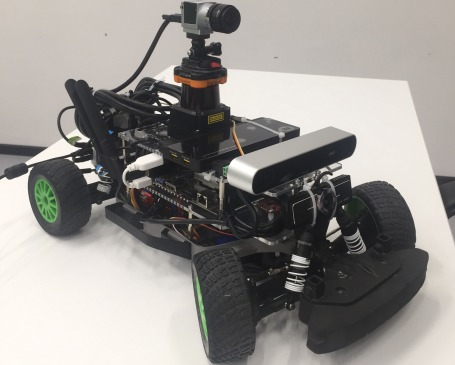
\includegraphics[width=0.5\textwidth]{pista}
                    
                    %\caption{Pista de corrida \cite{agostini2007}}
                \end{figure}
            %}
            \end{center}
        \end{columns}
%*----------- notes
    \note[item]{Notes can help you to remember important information. Turn on the notes option.}
\end{frame}
%-
%*----------- SLIDE -------------------------------------------------------------
\begin{frame}[c]{Objetivo} 
    %\framesubtitle{sub-objetivo}
    \transdissolve[duration=0.5]
   
    \begin{center}
        \Wider{%
        \begin{shaded}
        \begin{center}
            \vspace*{0.5cm}
            \resizebox{!}{0.5cm}{%
                \color{bg} Comparar as trajetórias de cada sistema SLAM
            }%
        \end{center}
        \end{shaded}
        }%
    \end{center}
    
   
%*----------- notes
    \note[item]{Notes can help you to remember important information. Turn on the notes option.}
\end{frame}
%-
{
%\setbeamertemplate{background}
%{\includegraphics[trim = 0 0 0 0, clip, width = \the\paperwidth, height = \the\paperheight]{marcel-knupfer-37wuETxVwTQ-unsplash.jpg}}
%*----------- SLIDE -------------------------------------------------------------
%\begin{frame}[c]{}
%    \transboxout[duration=0.5]
%    
%    \begin{columns}
%        \column{.1\textwidth}
%        \column{.3\textwidth}
%        \column{.53\textwidth}
%            \vspace*{-3.5cm}
%            \Huge{\textbf{\textcolor{mracula5}{Quando chovia...}}}
%    \end{columns}
%*----------- notes
%    \note[item]{Notes can help you to remember important information. Turn on the notes option.}
%\end{frame}
%-
}
%*----------- SLIDE -------------------------------------------------------------
\begin{frame}[t]{Lidar 2D}
    \transboxout[duration=0.5]
    %\framesubtitle{Darwin-OP}
    \begin{columns}
        %\column{.1\textwidth}
        \column{.4\textwidth}
            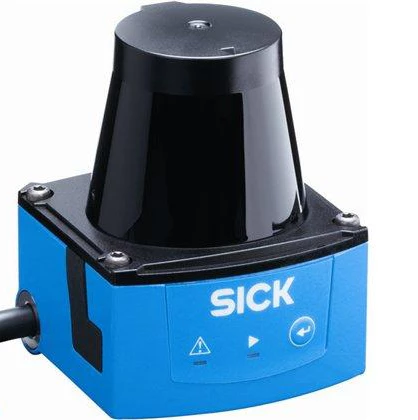
\includegraphics[width=0.9\textwidth]{lidar.png}
        \column{.4\textwidth}
            \begin{enumerate}
                \item GMAPPING;
                \item Hector SLAM;
                \item Cartographer;
                
            \end{enumerate}
    \end{columns}
 %*----------- notes
    %\note[item]{Notes can help you to remember important information. Turn on the notes option.}
\end{frame}
%-
%*----------- SLIDE -------------------------------------------------------------
\begin{frame}[c]{GMAPPING}
    %\transboxin[duration=1,direction=30]
    \centering

    \includemedia[
      width=0.7\linewidth,
      totalheight=0.39375\linewidth,
      activate=pageopen,
      passcontext, 
      addresource=./Source/movies/gmap.mp4,
      flashvars={
      source=./Source/movies/gmap.mp4
      &autoPlay=true
      &Loop=false}
      ]{\fbox{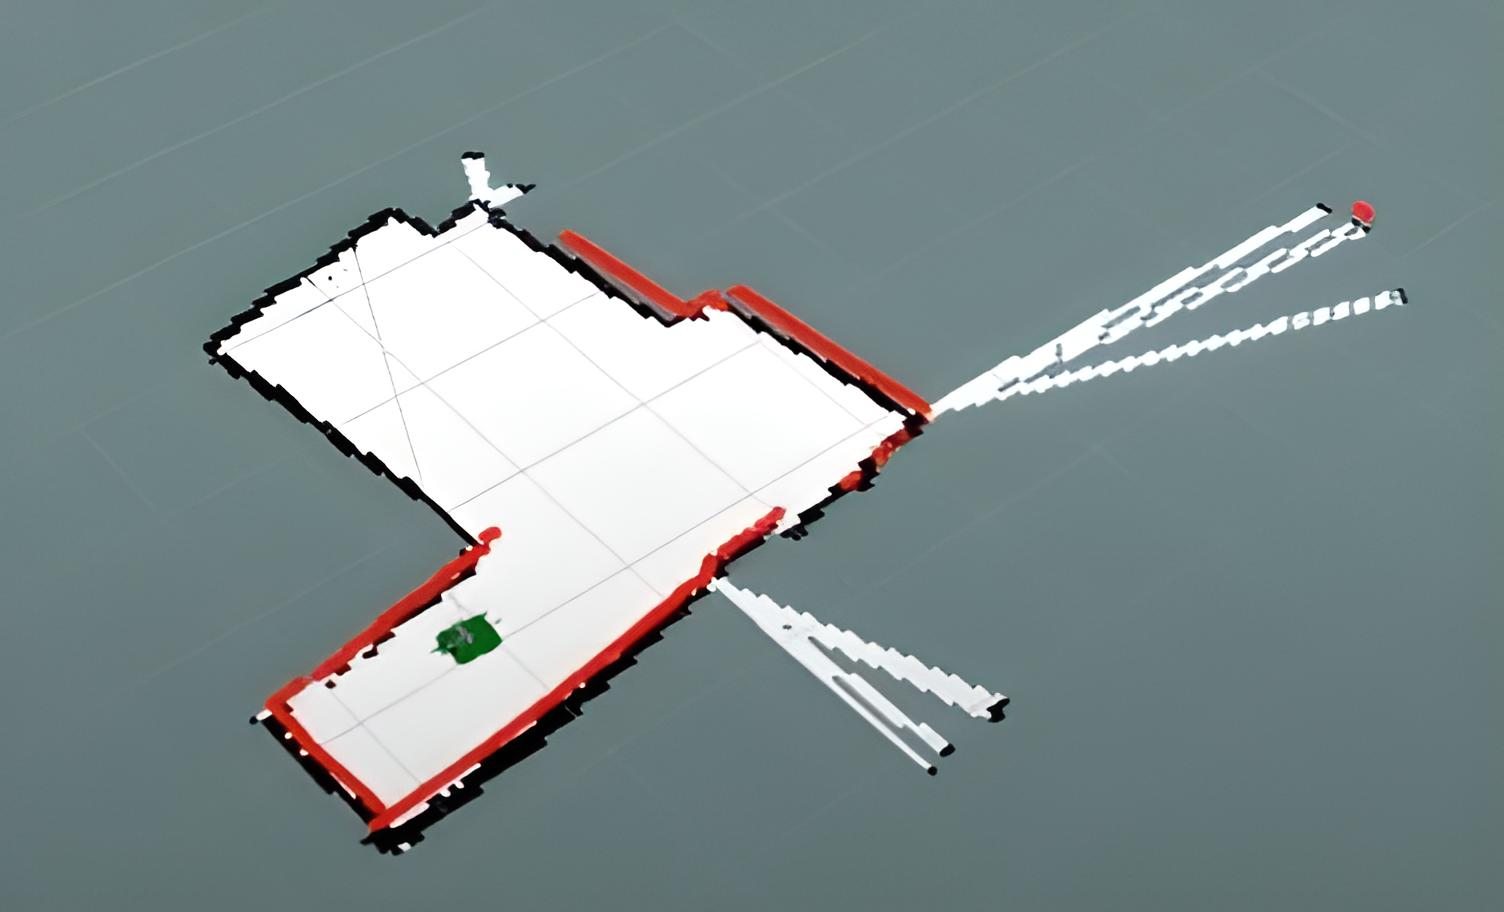
\includegraphics{gmap_v.png}}}{VPlayer.swf}

%*----------- notes
    %\note[item]{Notes can help you to remember important information. Turn on the notes option.}
\end{frame}
%-
%*----------- SLIDE -------------------------------------------------------------
\begin{frame}[c]{HECTOR SLAM}
    %\transboxin[duration=1,direction=30]
    \centering

    \includemedia[
      width=0.7\linewidth,
      totalheight=0.39375\linewidth,
      activate=pageopen,
      passcontext, 
      addresource=./Source/movies/HECTOR.mp4,
      flashvars={
      source=./Source/movies/HECTOR.mp4
      &autoPlay=true
      &Loop=false}
      ]{\fbox{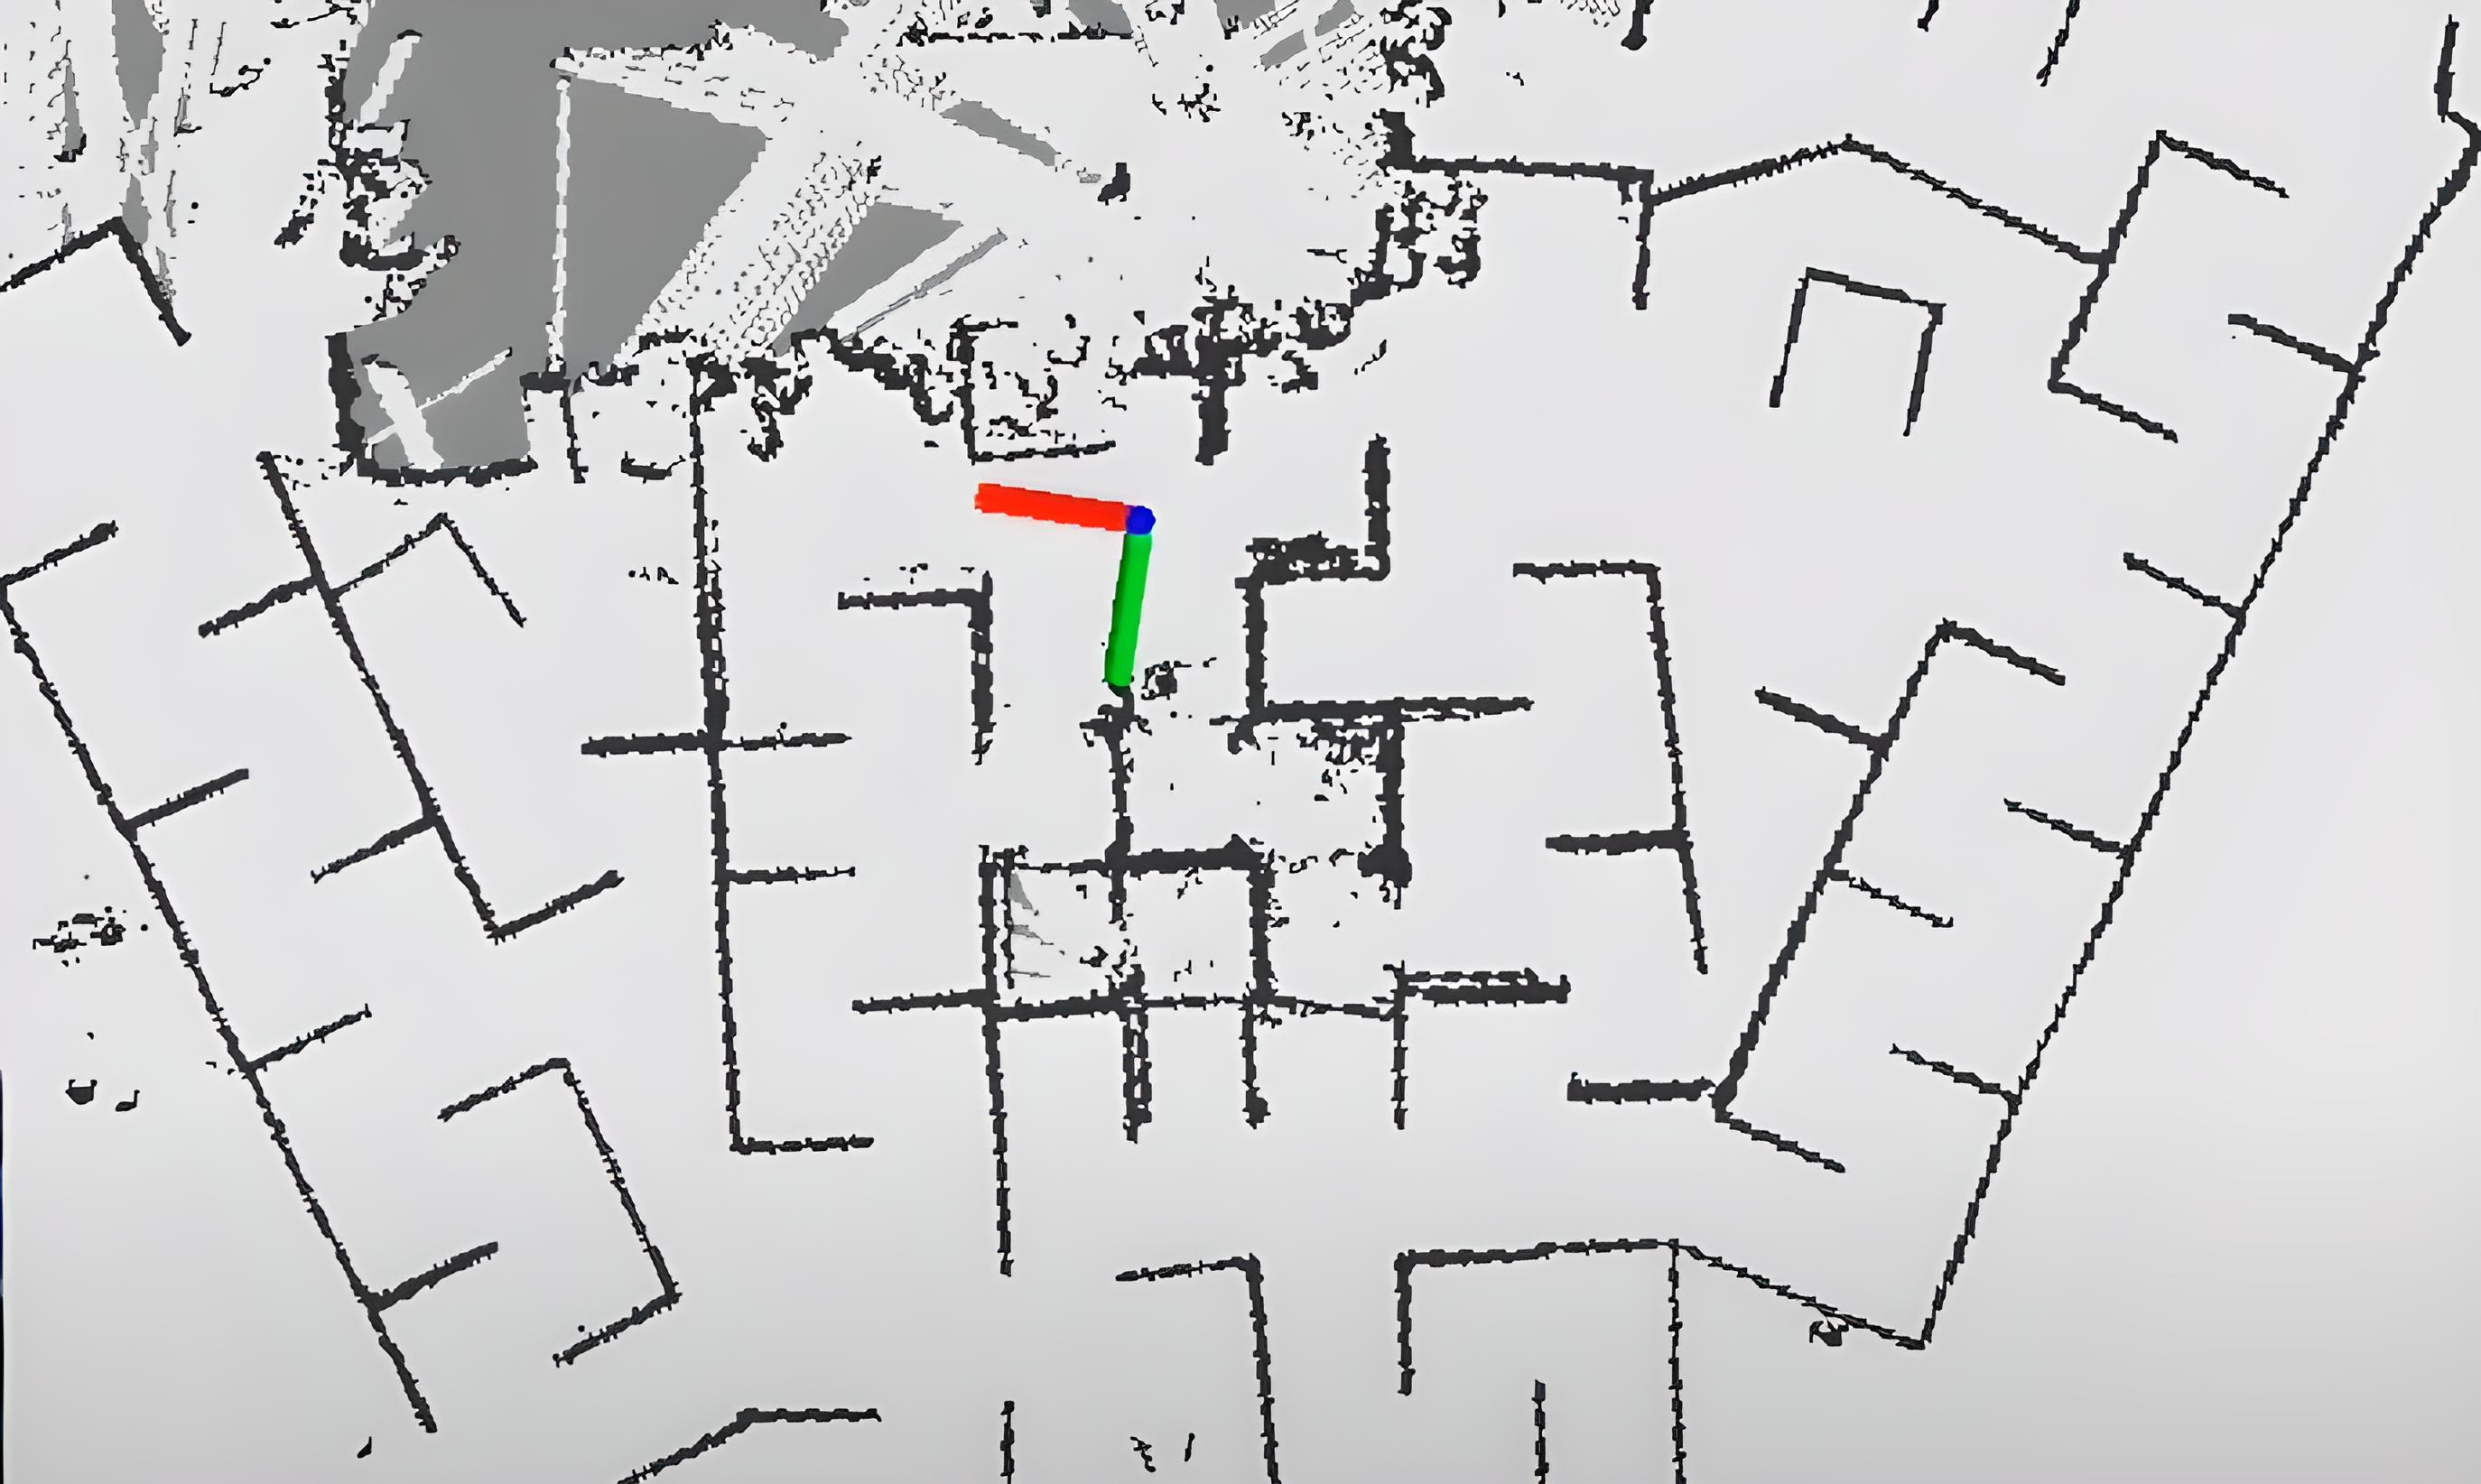
\includegraphics{hector.png}}}{VPlayer.swf}

%*----------- notes
    %\note[item]{Notes can help you to remember important information. Turn on the notes option.}
\end{frame}
%-

%*----------- SLIDE -------------------------------------------------------------
\begin{frame}[c]{CARTOGRAPHER}
    %\transboxin[duration=1,direction=30]
    \centering

    \includemedia[
      width=0.7\linewidth,
      totalheight=0.39375\linewidth,
      activate=pageopen,
      passcontext, 
      addresource=./Source/movies/Cartographer.mp4,
      flashvars={
      source=./Source/movies/Cartographer.mp4
      &autoPlay=true
      &Loop=false}
      ]{\fbox{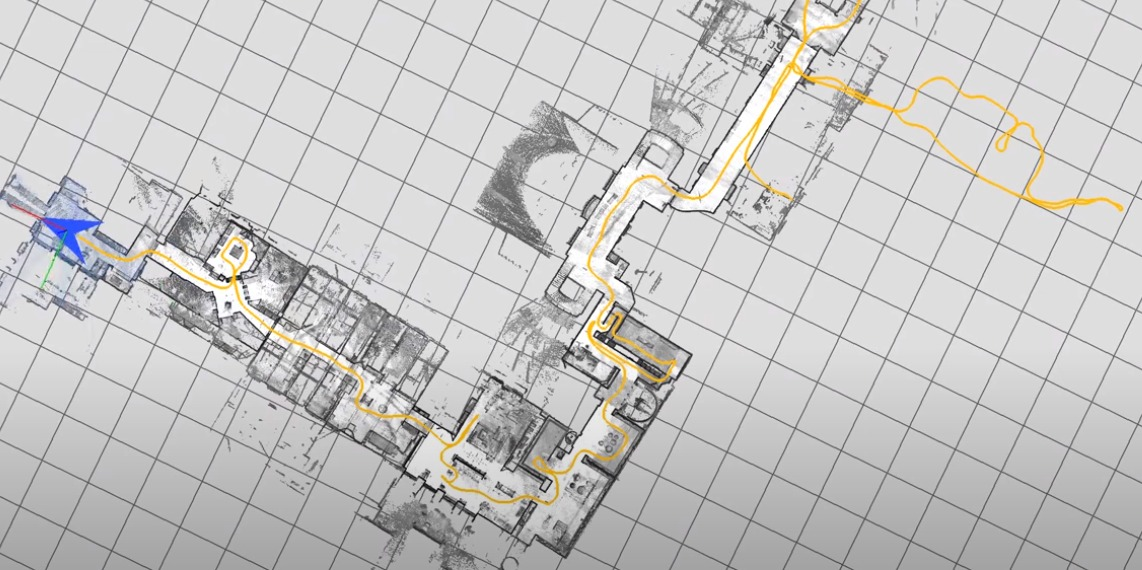
\includegraphics{cartographer.jpeg}}}{VPlayer.swf}

%*----------- notes
    %\note[item]{Notes can help you to remember important information. Turn on the notes option.}
\end{frame}
%-
%*----------- SLIDE -------------------------------------------------------------
\begin{frame}[t]{Comparação}
    \transboxout[duration=0.5]
    %\framesubtitle{Darwin-OP}
    \begin{columns}
        \column{.2\textwidth}
            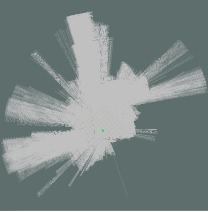
\includegraphics[width=1.2\textwidth]{gmapp.jpeg}
        \column{.2\textwidth}
            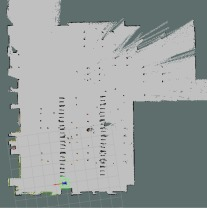
\includegraphics[width=1.2\textwidth]{hectorr.jpeg}
        \column{.2\textwidth}
            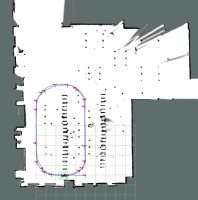
\includegraphics[width=1.2\textwidth]{cartog.jpeg}
        \column{.2\textwidth}
            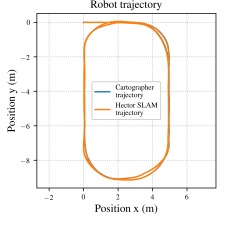
\includegraphics[width=1.2\textwidth]{hxc.jpeg}
    \end{columns}
 %*----------- notes
    %\note[item]{Notes can help you to remember important information. Turn on the notes option.}
\end{frame}
%-
%*----------- SLIDE -------------------------------------------------------------
\begin{frame}[t]{Lidar}
    \transboxout[duration=0.5]
    %\framesubtitle{Darwin-OP}
    \begin{columns}
        \column{.9\textwidth}
            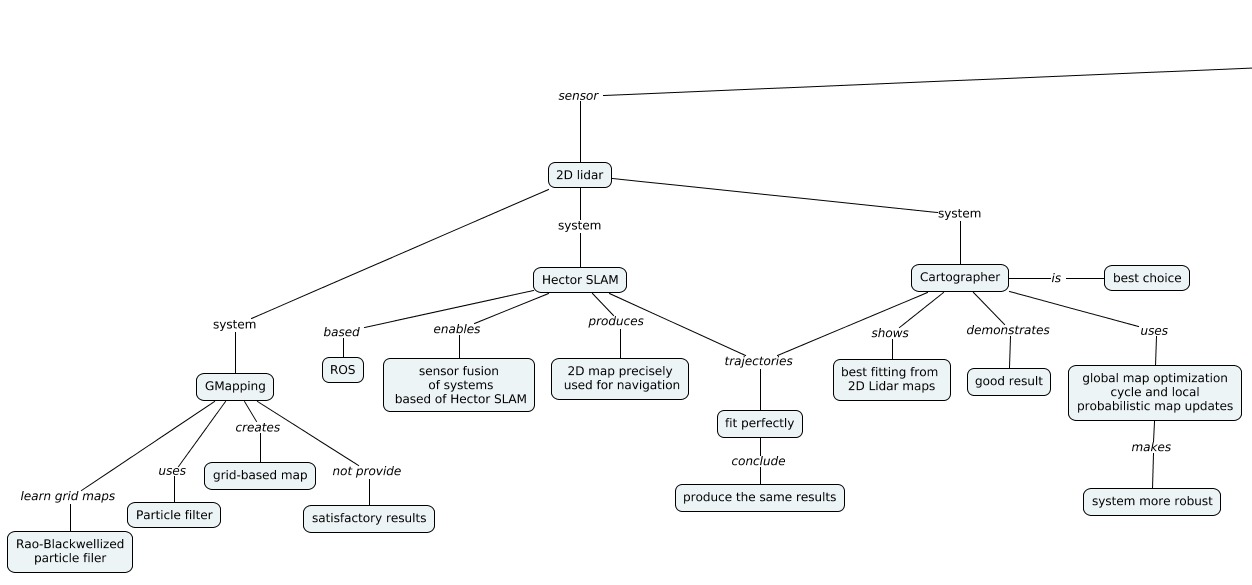
\includegraphics[width=1\textwidth]{mapalidar.jpeg}
    \end{columns}
 %*----------- notes
    %\note[item]{Notes can help you to remember important information. Turn on the notes option.}
\end{frame}
%-
%*----------- SLIDE -------------------------------------------------------------
\begin{frame}[t]{Monocular}
    \transboxout[duration=0.5]
    %\framesubtitle{Darwin-OP}
    \begin{columns}
        %\column{.1\textwidth}
        \column{.4\textwidth}
            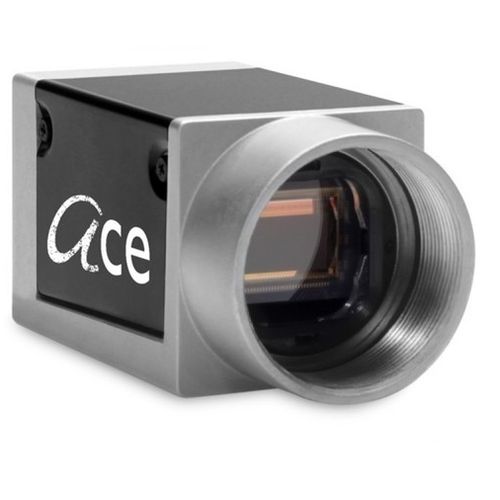
\includegraphics[width=0.9\textwidth]{cameramono.png}
        \column{.5\textwidth}
            \begin{enumerate}
                \item Parallel Tracking and Mapping (PTAM);
                \item Semi-direct Visual Odometry (SVO);
                \item Dense Piecewise Parallel Tracking and Mapping (DPP-
                        TAM);
                \item Large Scale Direct monocular SLAM (LSD SLAM);
                \item ORB SLAM (mono);
                \item Direct Sparse Odometry (DSO).
            \end{enumerate}
    \end{columns}
 %*----------- notes
    %\note[item]{Notes can help you to remember important information. Turn on the notes option.}
\end{frame}
%-
%*----------- SLIDE -------------------------------------------------------------
\begin{frame}[c]{Parallel Tracking and Mapping (PTAM):}
    %\transboxin[duration=1,direction=30]
    \centering

    \includemedia[
      width=0.7\linewidth,
      totalheight=0.39375\linewidth,
      activate=pageopen,
      passcontext, 
      addresource=./Source/movies/ptam.mp4,
      flashvars={
      source=./Source/movies/ptam.mp4
      &autoPlay=true
      &Loop=false}
      ]{\fbox{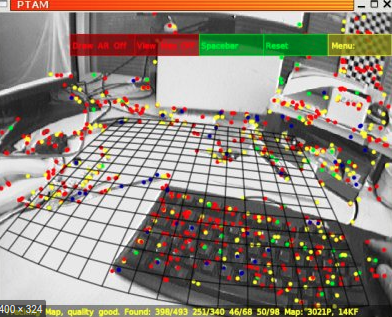
\includegraphics{ptam.png}}}{VPlayer.swf}

%*----------- notes
    %\note[item]{Notes can help you to remember important information. Turn on the notes option.}
\end{frame}
%-
%*----------- SLIDE -------------------------------------------------------------
\begin{frame}[c]{Semi-direct Visual Odometry (SVO):}
    %\transboxin[duration=1,direction=30]
    \centering

    \includemedia[
      width=0.7\linewidth,
      totalheight=0.39375\linewidth,
      activate=pageopen,
      passcontext, 
      addresource=./Source/movies/svo.mp4,
      flashvars={
      source=./Source/movies/svo.mp4
      &autoPlay=true
      &Loop=false}
      ]{\fbox{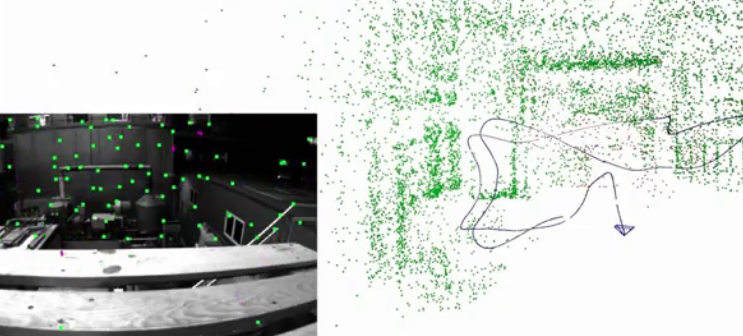
\includegraphics{svo.png}}}{VPlayer.swf}

%*----------- notes
    %\note[item]{Notes can help you to remember important information. Turn on the notes option.}
\end{frame}
%-
%*----------- SLIDE -------------------------------------------------------------
\begin{frame}[c]{Dense Piecewise Parallel Tracking and Mapping(DPP-
TAM)}
    %\transboxin[duration=1,direction=30]
    \centering

    \includemedia[
      width=0.7\linewidth,
      totalheight=0.39375\linewidth,
      activate=pageopen,
      passcontext, 
      addresource=./Source/movies/DPP-TAM.mp4,
      flashvars={
      source=./Source/movies/DPP-TAM.mp4
      &autoPlay=true
      &Loop=false}
      ]{\fbox{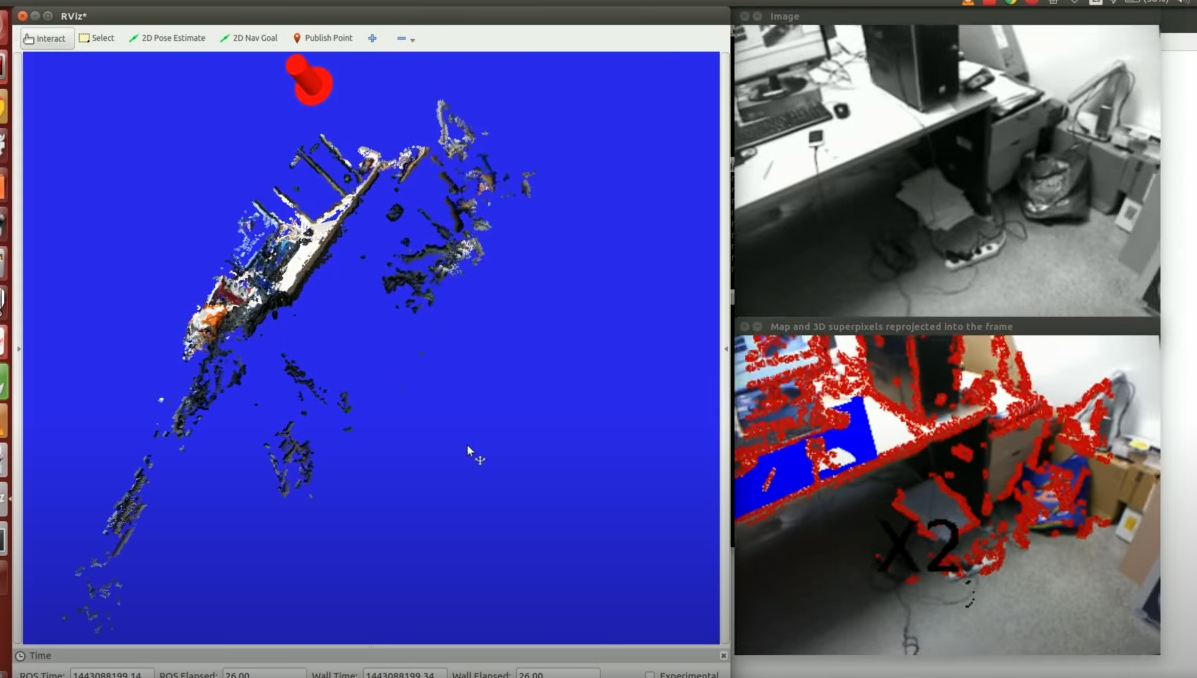
\includegraphics{DPP.png}}}{VPlayer.swf}

%*----------- notes
    %\note[item]{Notes can help you to remember important information. Turn on the notes option.}
\end{frame}
%-
%*----------- SLIDE -------------------------------------------------------------
\begin{frame}[c]{Large Scale Direct monocular SLAM (LSD SLAM)}
    %\transboxin[duration=1,direction=30]
    \centering

    \includemedia[
      width=0.7\linewidth,
      totalheight=0.39375\linewidth,
      activate=pageopen,
      passcontext, 
      addresource=./Source/movies/svo.mp4,
      flashvars={
      source=./Source/movies/svo.mp4
      &autoPlay=true
      &Loop=false}
      ]{\fbox{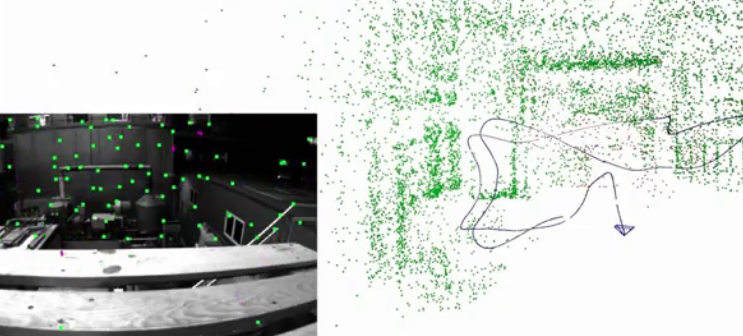
\includegraphics{svo.png}}}{VPlayer.swf}

%*----------- notes
    %\note[item]{Notes can help you to remember important information. Turn on the notes option.}
\end{frame}
%-
%*----------- SLIDE -------------------------------------------------------------
\begin{frame}[t]{O sistema robótico}
    \transboxout[duration=0.5]
    \framesubtitle{Darwin-OP}
    \begin{columns}
        \column{.1\textwidth}
        \column{.4\textwidth}
        \column{.4\textwidth}
    \end{columns}

    \begin{block}{Um bloco de destaque}
        Um exemplo de block.\\
        Oferece um certo destaque.
    \end{block}

    \begin{alertblock}{Um bloco de destaque}
        Um exemplo de alertblock.\\
        Oferece um certo destaque.
    \end{alertblock}

    \begin{exampleblock}{Um bloco de destaque}
        Um exemplo de exampleblock.
    \end{exampleblock}
 %*----------- notes
    \note[item]{Notes can help you to remember important information. Turn on the notes option.}
\end{frame}
%-
%*----------- SLIDE -------------------------------------------------------------
\begin{frame}[t]{O sistema robótico}
    \transboxout[duration=0.5]
    \framesubtitle{PlantUML}
    
    \tikzstyle{every node}=[draw=black,thick,anchor=west]
    \tikzstyle{selected}=[draw=red,fill=red!30]
    \tikzstyle{optional}=[dashed,fill=gray!50]

    \begin{tikzpicture}[%
        grow via three points={one child at (0.5,-0.7) and
        two children at (0.5,-0.7) and (0.5,-1.4)},
        edge from parent path={(\tikzparentnode.south) |- (\tikzchildnode.west)}]
        \node {texmf}
          child { node {doc}}		
          child { node {fonts}}
          child { node {source}}
          child { node [selected] {tex}
            child { node {generic}}
            child { node [optional] {latex}}
            child { node {plain}}
          }
          child [missing] {}				
          child [missing] {}				
          child [missing] {}				
          child { node {texdoc}};
      \end{tikzpicture}

 %*----------- notes
    \note[item]{Notes can help you to remember important information. Turn on the notes option.}
\end{frame}
%-
%*----------- SLIDE -------------------------------------------------------------
\begin{frame}[t]{O sistema robótico}
    \transboxout[duration=0.5]
    \framesubtitle{PlantUML}
    
    % Define block styles
    \tikzstyle{decision} = [diamond, draw, fill=blue!20, 
    text width=4.5em, text badly centered, node distance=3cm, inner sep=0pt]
    \tikzstyle{block} = [rectangle, draw, fill=blue!20, 
    text width=5em, text centered, rounded corners, minimum height=4em]
    \tikzstyle{line} = [draw, -latex']
    \tikzstyle{cloud} = [draw, ellipse,fill=red!20, node distance=3cm,
    minimum height=2em]

    \begin{tikzpicture}[node distance = 2cm, auto]
        % Place nodes
        \node [block] (init) {initialize model};
        \node [cloud, left of=init] (expert) {expert};
        \node [cloud, right of=init] (system) {system};
        \node [block, below of=init] (identify) {identify candidate models};
        \node [block, below of=identify] (evaluate) {evaluate candidate models};
        \node [block, left of=evaluate, node distance=3cm] (update) {update model};
        \node [decision, below of=evaluate] (decide) {is best candidate better?};
        \node [block, below of=decide, node distance=3cm] (stop) {stop};
        % Draw edges
        \path [line] (init) -- (identify);
        \path [line] (identify) -- (evaluate);
        \path [line] (evaluate) -- (decide);
        \path [line] (decide) -| node [near start] {yes} (update);
        \path [line] (update) |- (identify);
        \path [line] (decide) -- node {no}(stop);
        \path [line,dashed] (expert) -- (init);
        \path [line,dashed] (system) -- (init);
        \path [line,dashed] (system) |- (evaluate);
    \end{tikzpicture}

 %*----------- notes
    \note[item]{Notes can help you to remember important information. Turn on the notes option.}
\end{frame}
%-
%*----------- SLIDE -------------------------------------------------------------
\begin{frame}[t]{O sistema robótico}
    \transboxout[duration=0.5]
    \framesubtitle{PlantUML}
    
    \begin{tikzpicture}[line width=0.1pt]
        \draw(0,0) circle(5cm);
        \draw(0,0) circle(1cm);
        \draw(0,0) node {\Huge$\mathbf{A}$};
        \draw(0,0) circle(4.5cm);
        \draw(-48:2.5) arc(-48:240:2.5cm);
        %% The outer nodes
        \foreach \x in {36,72,...,360}
            \shade[ball color=black](\x:5) circle(4pt);
        \foreach \nodes in {12,24,...,360}
            \shade[ball color=black](\nodes:3.5) circle(4pt);
        %%% The connecting nodes
        \foreach \angle in {-48,-12,...,240}
            \draw(\angle:2.5) --++(\angle:0.9cm);
        %%% outer interconnects
        \foreach \angle in {-24,12,...,306}
            \draw(\angle:3.6) --++(\angle:0.9cm);
        \foreach \y in {-24,12,...,240}
            \shade[ball color=black](\y:4.5cm) circle(4pt);
    
        %% outer most connections
        \foreach \angle in{-36,0,...,306}
            \draw(\angle:4.9cm) --(\angle:4.7cm) [rotate=\angle]arc(0:180:0.20cm);
        \foreach \angle in{-36,0,...,306}
            \draw(\angle:4.3cm) --(\angle:3.6cm);
        %% Outer connects and leads
        \shade[ball color=black](276:6) circle(4pt);
        \draw(276:6)circle(4pt)--(276:5.2)[rotate=276]arc(0:180:0.25cm);
        \draw(276:7)node {$\mathbf{K_0}$};
        \draw(276:4.2)[rotate=276]arc(180:360:0.25cm);
        \draw(276:4.2)--(276:3.5);
    
        %% Exploitation of circular symmetry of the required figure
    
        {[rotate=72]
            \shade[ball color=black](276:6) circle(4pt);
            \draw(276:6)circle(4pt)--(276:5.2)[rotate=276]arc(0:180:0.25cm);
            \draw(270:6)node {$\mathbf{K_1-K_9}$};
            \draw(276:4.2)[rotate=276]arc(180:360:0.25cm);%%%
            \draw(276:4.2)--(276:3.5);
        }
    
        {[rotate=-48]
            \shade[ball color=black](276:6) circle(4pt);
            \draw(276:6)circle(4pt)--(276:5.2)[rotate=276]arc(0:180:0.20cm);
            \draw(276:7)node {$\mathbf{g_2}$};
            \draw(276:4.8)--(276:4.5);
        }
    
        \draw(180:5)--(180:6);
        \shade[ball color=black](180:6) circle(4pt);
        \draw(180:6.5)node{$\mathbf{g_1}$};
    \end{tikzpicture}

 %*----------- notes
    \note[item]{Notes can help you to remember important information. Turn on the notes option.}
\end{frame}
%-

 % %*----------- SLIDE -------------------------------------------------------------
% \begin{frame}[c]{A tropa dos quatro incríveis}
%     %\transboxin[duration=1,direction=30]
%     A simulação deverá ser desenvolvida com 4 unidades Darwin-OP, comumente esta unidade é utilizada para desafios em competições de robótica.
%     \newline

%     A tropa será composta por 4 Darwin-OP, e deverá realizar duas missões:
%     \begin{itemize}
%         \item marchar em forma unida em linha;
%         \item realizar corrida de revezamento.
%     \end{itemize}

%     \begin{figure}
%         \includegraphics[trim = 0 20 0 50, clip, width=0.8\textwidth]{darwin-op-sequencia}
%         %\caption{.}
%     \end{figure}
% %*----------- notes
%     \note[item]{Notes can help you to remember important information. Turn on the notes option.}
% \end{frame}
% %-
% %*----------- SLIDE -------------------------------------------------------------
% \begin{frame}[t]{Algumas regras}
%     \begin{itemize}
%         \item A marcha deverá ser realizada diante de um percurso de 2 metros.
%         \item A marcha e a corrida de revezamento deverão serem realizadas numa pista de corrida;
%         \item A corrida deverá ser realizada numa pista de 8 metros;
%         \item Cada Darwin-OP deverá percorrer 2 metros para realizar o revezamento;
%         \item A região de revezamento deverá ser uma área de até 0.4 metros;
%         \item O conceito para o revezamento será o de alinhar-se os dois Darwin-OP durante até 15 segundos a uma distância de no máximo 0.2 metros entre ambos, ou seja será considerado passagem de bastão quando os dois Darwin-OP passarem 15 segundos com movimentos sincronizados a uma distância máxima de 0.2 metros dentro da região de revezamento;
%         \item A pista de corrida deverá ser considerada analogamente a uma pista real;
%         \item A lateral da pista deverá ter lados de 2 metros;
%         \item Considerar sempre os critérios de uma corrida de revezamento.
%     \end{itemize}
   
%     % \begin{columns}[t]
%     %     \column{.45\textwidth}
%     %         detalhar sistemas em subconjuntos\\
%     %         listar possíveis modos de falhas\\
%     %         analisar cada modo de falha, juntamente com suas possíveis causas e sintomas
%     %     \column{.45\textwidth}
%     %         estimar os efeitos de cada modo de falhas\\
%     %         estimar a criticidade de cada efeito\\
%     %         identificar ações para minimizar falhas
%     % \end{columns}
% %*----------- notes
%     \note[item]{Notes can help you to remember important information. Turn on the notes option.}
% \end{frame}
% %-
% %*----------- SLIDE -------------------------------------------------------------
% \begin{frame}[c]{A pista}
%     \begin{figure}
%         %\includegraphics[width=0.7\textwidth]{pista_corrida}
       
%         \roundpic[xshift=0cm,yshift=0cm]{3cm}{7cm}{pista_corrida}
          
%         \caption{Formato de um pista de corrida.\cite{agostini2007}}
%     \end{figure}
% %*----------- notes
%     \note[item]{Notes can help you to remember important information. Turn on the notes option.}
% \end{frame}
% %-
 % %*----------- SLIDE -------------------------------------------------------------
% \begin{frame}[t]{As lideranças das equipes dos Novos Talentos}
%     \vspace{0.5cm}
%     \begin{columns}
%         \column{.01\textwidth}
%         \column{.7\textwidth}
%             \begin{itemize}
%                 \item equipe \tikznode{cmark}{RAJA} será liderada por Aziel Freitas
%                 \item equipe \Circled[outer color=mracula8, inner ysep=8pt]{BORG} será liderada por Mateus Cerqueira.
%                 \item equipe \Circled[outer color=mracula7, inner ysep=8pt]{BORG} será liderada por Mateus Cerqueira.
%                 \item equipe \Circled[outer color=mracula9, inner ysep=8pt]{jerotimon} será liderada por Mateus Cerqueira.
%                 \item equipe TIMON-HM será liderada por Leonardo Lima.
%             \end{itemize}
%         \column{.29\textwidth}
%             \includegraphics[width=.9\textwidth, trim={10cm 0 10cm 0},clip]{equipe}
%     \end{columns}
%     \vspace{1cm}
    
%     \emph{Para este desafio não será cobrado o relatório técnico, porém o acompanhamento deverá seguir o mesmo ritmo dos desafios anteriores.}

%     %add circle on word
%     \begin{tikzpicture}[remember picture,overlay]
%         \draw[mracula5,very thick] (cmark) circle[x radius=8mm,y radius=4mm]; 
%     \end{tikzpicture}
% %*----------- notes
%     \note[item]{Notes can help you to remember important information. Turn on the notes option.}
% \end{frame}
% %-
% %*----------- SLIDE -------------------------------------------------------------
% \begin{frame}[t]{O progresso das equipes}
%     Um dos indicadores para o acompanhamento das equipes será o percentual de conclusão geral da equipe.
%     O planejamento das atividades deverá seguir a metodologia aplicada no desenvolvimento de projetos de robótica.
%     \newline
%     %\vspace{0.5cm}
%     \begin{table}[ht!]
%     \centering
%         \caption{PERCENTUAL DE CONCLUSÃO POR EQUIPE}
%         \begin{tabular}{|l|c|c|c|c|} \hline
%             \textbf{EQUIPE}&\textbf{04/05}&\textbf{11/05}&\textbf{18/05}&\textbf{25/05}\\ \hline
%             RAJA & 17\% &32\% & &  \\ \hline
%             BORG & 0\% &41\% & &  \\ \hline
%             TIMON-HM & 5\% &47\% & &  \\ \hline
%         \end{tabular}
%     \end{table}
% %*----------- notes
%     \note[item]{Notes can help you to remember important information. Turn on the notes option.}
% \end{frame}
% %-
% %*----------- SLIDE -------------------------------------------------------------
% \begin{frame}[t]{O progresso das equipes}
%     Um dos indicadores para o acompanhamento das equipes será o percentual de conclusão geral da equipe.
%     O planejamento das atividades deverá seguir a metodologia aplicada no desenvolvimento de projetos de robótica.
%     \newline
%     %\vspace{0.5cm}
%     % \begin{table}[ht!]
%     % \centering
%     %     \caption{PERCENTUAL DE CONCLUSÃO POR EQUIPE}
%     %     \begin{tabular}{|l|c|c|c|c|} \hline
%     %         \textbf{EQUIPE}&\textbf{04/05}&\textbf{11/05}&\textbf{18/05}&\textbf{25/05}\\ \hline
%     %         RAJA & 17\% &32\% & &  \\ \hline
%     %         BORG & 0\% &41\% & &  \\ \hline
%     %         TIMON-HM & 5\% &47\% & &  \\ \hline
%     %     \end{tabular}
%     % \end{table}
% %*----------- notes
%     \note[item]{Notes can help you to remember important information. Turn on the notes option.}
% \end{frame}
% %-
% %*----------- SLIDE -------------------------------------------------------------
% \begin{frame}[t]{O progresso das equipes}
%     Um dos indicadores para o acompanhamento das equipes será o percentual de conclusão geral da equipe.
%     O planejamento das atividades deverá seguir a metodologia aplicada no desenvolvimento de projetos de robótica.
%     \newline
%     %\vspace{0.5cm}
%     % \begin{table}[ht!]
%     % \centering
%     %     \caption{PERCENTUAL DE CONCLUSÃO POR EQUIPE}
%     %     \begin{tabular}{|l|c|c|c|c|} \hline
%     %         \textbf{EQUIPE}&\textbf{04/05}&\textbf{11/05}&\textbf{18/05}&\textbf{25/05}\\ \hline
%     %         RAJA & 17\% &32\% & &  \\ \hline
%     %         BORG & 0\% &41\% & &  \\ \hline
%     %         TIMON-HM & 5\% &47\% & &  \\ \hline
%     %     \end{tabular}
%     % \end{table}
    
%     \url{https://braziliansinrobotics.com/}
% %*----------- notes
%     \note[item]{Notes can help you to remember important information. Turn on the notes option.}
% \end{frame}
% %-
 % %*----------- SLIDE -------------------------------------------------------------
% \begin{frame}[t]{Finalização}
%     \begin{itemize}
%         \item Cada líder deverá realizar a apresentação final do desafio no dia 25/maio/2020.
%         \item No dia da apresentação, somente o líder poderá responder os questionamentos emitidos pelos facilitadores.
%         \item A avaliação será da equipe, não havendo avaliação individual dos integrantes da equipe com exceção do líder de cada equipe.
%         \item A apresentação deverá ser desenvolvida em latex.
%         \item Os videos dos desafios deverão estar contidos na apresentação final.
%         \item Os videos deverão ser completos, tendo começo, meio e fim da missão realizada.
%     \end{itemize}
% %*----------- notes
%     \note[item]{Notes can help you to remember important information. Turn on the notes option.}
% \end{frame}
% %-
% %*----------- SLIDE -------------------------------------------------------------
% \begin{frame}[c]{A importância atual da robótica}
%     \begin{center}
    
%         \includemedia[
%             width=0.7\linewidth,
%             totalheight=0.39375\linewidth,
%             activate=pageopen,
%             passcontext, 
%             %transparent,
%             addresource=./Source/gifs/robotdesinfec.wmv,
%             flashvars={
%             source=./Source/gifs/robotdesinfec.wmv
%             &autoPlay=true
%             &autoRewind=true
%             &loop=true}
%             ]{\fbox{\includegraphics{Source/gifs/robotdesinfec0.png}}}{VPlayer.swf}
%     \end{center}

% %*----------- notes
%     \note[item]{Notes can help you to remember important information. Turn on the notes option.}
%  \end{frame}
% %-
% %*----------- SLIDE -------------------------------------------------------------
% \begin{frame}[fragile]{A importância atual da robótica}
%     Para a implentação de R gráficos deve-se realizar os seguintes comando no ambiente R:

%     \begin{lstlisting}[language=R]
%         library(tikzDevice)
%         beamer.parms = list(paperwidth   = 364.19536/72,
%                     paperheight  = 273.14662/72,
%                     textwidth    = 307.28987/72,
%                     textheight   = 269.14662/72)
%         tikz("./your_file.tex", 
%             width = beamer.parms$textwidth, 
%             height = beamer.parms$textheight)
%         ggqqplot(na.omit(my_data$col2))
%         dev.off()
%     \end{lstlisting}

%     \begin{columns}
%         \column{.01\textwidth}
%         \column{.59\textwidth}
%             \textbf{A penúltima linha do texto acima é o códifo em R para a construção do gráfico.}
                
%         \column{.4\textwidth}
%             \centering
%             \begin{tikzpicture}[thick, scale=0.4, every node/.style={scale=0.1}]
%                 \node[at=(current page.center)] {
%                %\input{./Media/r-graphics/img-marco1.tex}
%                 \input{./Source/r-graphics/graficox.tex}
%                 };
%             \end{tikzpicture}
%     \end{columns}
% %*----------- notes
%     \note[item]{Notes can help you to remember important information. Turn on the notes option.}
%  \end{frame}
% %-
% %*----------- SLIDE -------------------------------------------------------------
% \begin{frame}[c]{A importância atual da robótica}
%     \centering
%     \framesubtitle{robo}
%     \begin{bclogo}[ 
%         couleur=white!10!white,
%         ombre=false,
%         epBord=3,
%         couleurBord = gcolor,
%         arrondi = 0.2,
%         logo=\bcinfo]{}
%         \centering
%         \begin{tikzpicture}[thick, scale=0.35, every node/.style={scale=0.5}]
%             \node[at=(current page.center)] {
%             \input{./Source/r-graphics/graficox.tex}
%             };
%         \end{tikzpicture}
%     \end{bclogo}
% %*----------- notes
%     \note[item]{Notes can help you to remember important information. Turn on the notes option.}
%  \end{frame}
%  %-
% %*----------- SLIDE -------------------------------------------------------------
% \begin{frame}
%     \begin{center}
%         \vspace*{1.5cm}
%         \textbf{\Huge{\textcolor{mracula5}{MUDANÇA}}}
%     \end{center}
    
% %*----------- notes
%     \note[item]{Notes can help you to remember important information. Turn on the notes option.}
%  \end{frame}
%  %-
% %*----------- SLIDE -------------------------------------------------------------
% \begin{frame}
%     %\transdissolve[duration=0.5]
%     %\hspace*{-1cm}
%     \begin{columns}
%         %\column{.01\textwidth}
%         \column{0.4\textwidth}
%             ~\hfill
%             \vbox{}\vskip-1.4ex%
%             \begin{beamercolorbox}[sep=8em, colsep*=18pt, center, wd=\textwidth, ht=\paperheight]{title page header}%
%                 \begin{center}
%                     \textbf{\huge{VISÃO}}\par
%                     \vspace*{0.3cm}
%                     \textbf{\huge{DO}}\par
%                     \vspace*{0.3cm}
%                     \textbf{\huge{FUTURA}}
%                 \end{center}
%             \end{beamercolorbox}%
%         \hfill\hfill
%         \column{.05\textwidth} 
%         \column{.6\textwidth}
%             \small{\lipsum[2-1]}
%             \begin{itemize}
%                 \item tópico 1
%                 \item tópico 2 
%                 \item \xout{tópico 3}
%                 \item \sout{last tópico}
%             \end{itemize}
%     \end{columns}
  
%  %*----------- notes__
%     \note[item]{Notes can help you to remember important information. Turn on the notes option.}
% \end{frame}
% %-
% %*----------- SLIDE -------------------------------------------------------------
% \begin{frame}
%     %\transdissolve[duration=0.5]
%     %\hspace*{-1cm}
%     \begin{columns}
%         %\column{.01\textwidth}
%         \column{0.4\textwidth}
%        %~\hfill
%         %\begin{beamercolorbox}[sep=8em, colsep*=18pt, center, wd=\textwidth, ht=\paperheight]{title page header}%
%         %\vspace*{-1.5cm}%
%         % \raggedright
%         % \begin{figure}[p]
%         %     \includegraphics[trim = 0 0 0 10, clip, width=1.03\paperwidth, height=1.03\paperheight, keepaspectratio=true]{melody-p-wFN9B3s_iik-unsplash.jpg}
%         % \end{figure}

%         \begin{tikzpicture}[remember picture,overlay]
%             \node [xshift=3cm,yshift=-4.1cm] at (current page.north west) {
%                 \includegraphics[width=\paperwidth, height=\paperheight, keepaspectratio]{melody-p-wFN9B3s_iik-unsplash.jpg}
%             };
%         \end{tikzpicture}
%         %\end{beamercolorbox}%
%         %\hfill\hfill
%         \column{.05\textwidth} 
%         \column{.6\textwidth}
%             \small{\lipsum[2-1]}
%             \begin{itemize}
%                 \item tópico 1
%                 \item tópico 2 
%                 \item \xout{tópico 3}
%                 \item \sout{last tópico}
%             \end{itemize}
%     \end{columns}
  
%  %*----------- notes__
%     \note[item]{Notes can help you to remember important information. Turn on the notes option.}
% \end{frame}
% %-
% %*----------- SLIDE -------------------------------------------------------------
% \begin{frame}
%     %\transdissolve[duration=0.5]
%     %\hspace*{-1cm}
%     \begin{columns}
%         %\column{.01\textwidth}
%         \hspace*{0.5cm}
%         \column{.6\textwidth}
%             \small{\lipsum[2-1]}
%             \begin{itemize}
%                 \item tópico 1
%                 \item tópico 2 
%                 \item \xout{tópico 3}
%                 \item \sout{last tópico}
%             \end{itemize}
%         \column{.05\textwidth} 
%         \column{0.4\textwidth}
%             ~\hfill
%             \vbox{}\vskip-1.4ex%
%             \begin{beamercolorbox}[sep=8em, colsep*=18pt, center, wd=\textwidth, ht=\paperheight]{title page header}%
%                 \begin{center}
%                     \textbf{\huge{VISÃO}}\par
%                     \vspace*{0.3cm}
%                     \textbf{\huge{FUTURA}}
%                 \end{center}
%             \end{beamercolorbox}%
%         \hfill\hfill
%     \end{columns}
  
%  %*----------- notes__
%     \note[item]{Notes can help you to remember important information. Turn on the notes option.}
% \end{frame}
% %-
% %*----------- SLIDE -------------------------------------------------------------
% \begin{frame}
%     %\transdissolve[duration=0.5]
%     %\hspace*{-1cm}
    
%     \begin{columns}
%         %\column{.01\textwidth}
%         \column{0.4\textwidth}
%             ~\hfill
%             \vbox{}\vskip-1.4ex%
%             \begin{beamercolorbox}[sep=8em, colsep*=18pt, wd=\textwidth,ht=\paperheight]{title page header}
%                 \begin{center}
%                     \textbf{\huge{VISÃO}}\par
%                     \vspace*{0.3cm}
%                     \textbf{\huge{FUTURA}}
%                 \end{center}
%             \end{beamercolorbox}%
%         \column{.05\textwidth} 
%         \column{.6\textwidth}
%         \begin{center}
%             \begin{figure}
%                 \includegraphics[width=.5\textwidth]{darwin-op-2}
%                 \caption{Darwim OP \cite{webcite}}
%             \end{figure}
            
%         \end{center}
            
%     \end{columns}
  
%  %*----------- notes
%     \note[item]{Notes can help you to remember important information. Turn on the notes option.}
% \end{frame}
%  %-
% %*----------- SLIDE -------------------------------------------------------------
% \begin{frame}
%     %\transdissolve[duration=0.5]
%     %\hspace*{-1cm}
    
%     \begin{columns}
%         %\column{.01\textwidth}
%         \column{.6\textwidth}
%             \begin{center}
%                 \begin{figure}
%                     \includegraphics[width=.5\textwidth]{darwin-op-2}
%                     \caption{Darwim OP \cite{webcite}}
%                 \end{figure}
                
%             \end{center}
%         \column{.05\textwidth}
%         \column{0.4\textwidth}
%             ~\hfill
%             \vbox{}\vskip-1.4ex%
%             \begin{beamercolorbox}[sep=8em, colsep*=18pt, wd=\textwidth,ht=\paperheight]{title page header}
%                 \begin{center}
%                     \textbf{\huge{VISÃO}}\par
%                     \vspace*{0.3cm}
%                     \textbf{\huge{FUTURA}}
%                 \end{center}
%             \end{beamercolorbox}%
%     \end{columns}
  
%  %*----------- notes
%     \note[item]{Notes can help you to remember important information. Turn on the notes option.}
% \end{frame}
% %-
% %*----------- SLIDE -------------------------------------------------------------
% % \begin{frame}
% %     %\transdissolve[duration=0.5]
% %     %\hspace*{-1cm}
    
% %     \begin{columns}
% %         %\column{.01\textwidth}
% %         \column{.6\textwidth}
% %             \begin{tikzpicture}[node distance=1.cm, every node/.style={fill=white, font=\sffamily}, align=center]
% %             % Specification of nodes (position, etc.)
% %                 \node (start)             [activityStarts]              {Activity starts};
% %                 \node (onCreateBlock)     [process, below of=start]          {onCreate()};
% %                 \node (onStartBlock)      [process, below of=onCreateBlock]   {onStart()};
% %                 \node (onResumeBlock)     [process, below of=onStartBlock]   {onResume()};
% %                 \node (activityRuns)      [activityRuns, below of=onResumeBlock] {Activity is running};
% %                 \node (onPauseBlock)      [process, below of=activityRuns, yshift=-1cm] {onPause()};
% %                 \node (onStopBlock)       [process, below of=onPauseBlock, yshift=-1cm] {onStop()};
% %                 \node (onDestroyBlock)    [process, below of=onStopBlock, yshift=-1cm] {onDestroy()};
% %                 \node (onRestartBlock)    [process, right of=onStartBlock, xshift=4cm] {onRestart()};
% %                 \node (ActivityEnds)      [startstop, left of=activityRuns, xshift=-4cm] {Process is killed};
% %                 \node (ActivityDestroyed) [startstop, below of=onDestroyBlock] {Activity is shut down};     
% %                 % Specification of lines between nodes specified above
% %                 % with aditional nodes for description 
% %                 \draw[->]             (start) -- (onCreateBlock);
% %                 \draw[->]     (onCreateBlock) -- (onStartBlock);
% %                 \draw[->]      (onStartBlock) -- (onResumeBlock);
% %                 \draw[->]      (activityRuns) -- node[text width=4cm] {Another activity comes in front of the activity} (onPauseBlock);
% %                 \draw[->]      (onPauseBlock) -- node {The activity is no longer visible} (onStopBlock);
% %                 \draw[->]       (onStopBlock) -- node {The activity is shut down by user or system} (onDestroyBlock);
% %                 \draw[->]    (onRestartBlock) -- (onStartBlock);
% %                 \draw[->]       (onStopBlock) -| node[yshift=1.25cm, text width=3cm]
% %                                                 {The activity comes to the foreground}
% %                                                 (onRestartBlock);
% %                 \draw[->]    (onDestroyBlock) -- (ActivityDestroyed);
% %                 \draw[->]      (onPauseBlock) -| node(priorityXMemory)
% %                                                 {higher priority $\rightarrow$ more memory}
% %                                                 (ActivityEnds);
% %                 \draw           (onStopBlock) -| (priorityXMemory);
% %                 \draw[->]     (ActivityEnds)  |- node [yshift=-2cm, text width=3.1cm]
% %                                                     {User navigates back to the activity}
% %                                                     (onCreateBlock);
% %                 \draw[->] (onPauseBlock.east) -- ++(2.6,0) -- ++(0,2) -- ++(0,2) --                
% %                     node[xshift=1.2cm,yshift=-1.5cm, text width=2.5cm]
% %                     {The activity comes to the foreground}(onResumeBlock.east);
% %             \end{tikzpicture}
% %         \column{.05\textwidth}
% %         \column{0.4\textwidth}
% %             ~\hfill
% %             \vbox{}\vskip-1.4ex%
% %             \begin{beamercolorbox}[sep=8em, colsep*=18pt, wd=\textwidth,ht=\paperheight]{title page header}
% %                 \begin{center}
% %                     \textbf{\huge{VISÃO}}\par
% %                     \vspace*{0.3cm}
% %                     \textbf{\huge{FUTURA}}
% %                 \end{center}
% %             \end{beamercolorbox}%
% %     \end{columns}
  
% %  %*----------- notes
% %     \note[item]{Notes can help you to remember important information. Turn on the notes option.}
% % \end{frame}
% %-
% %*----------- SLIDE -------------------------------------------------------------
% \begin{frame}{}
%     %\transdissolve[duration=0.5]
%     %\hspace*{-1cm}
    
%     \begin{columns}
%         %\column{.01\textwidth}
%         \column{.6\textwidth}
%         \begin{tikzpicture}[font=\sffamily, every matrix/.style={ampersand replacement=\&,column sep=1cm,row sep=1cm}, source/.style={draw,thick,rounded corners,fill=yellow!20,inner sep=.3cm},process/.style={draw,thick,circle,fill=blue!20}, sink/.style={source,fill=green!20},datastore/.style={draw,very thick,shape=datastore,inner sep=.3cm}, dots/.style={gray,scale=2}, to/.style={->,>=stealth',shorten >=1pt,semithick,font=\sffamily\footnotesize}, every node/.style={align=center}]
          
%             % Position the nodes using a matrix layout
%             \matrix{
%               \node[source] (hisparcbox) {electronics};
%                 \& \node[process] (daq) {DAQ}; \& \\
%                 \& \node[datastore] (buffer) {buffer}; \& \\
%                 \node[datastore] (storage) {storage};
%                 \& \node[process] (monitor) {monitor};
%                 \& \node[sink] (datastore) {datastore}; \\
%             };
          
%             % Draw the arrows between the nodes and label them.
%             \draw[to] (hisparcbox) -- node[midway,above] {raw events} node[midway,below] {level 0} (daq);
%             \draw[to] (daq) -- node[midway,right] {raw event data\\level 1} (buffer);
%             \draw[to] (buffer) -- node[midway,right] {raw event data\\level 1} (monitor);
%             \draw[to] (monitor) to[bend right=50] node[midway,above] {events} node[midway,below] {level 1} (storage);
%             \draw[to] (storage) to[bend right=50] node[midway,above] {events} node[midway,below] {level 1} (monitor);
%             \draw[to] (monitor) -- node[midway,above] {events} node[midway,below] {level 1} (datastore);
%           \end{tikzpicture}
                
        
%         \column{.05\textwidth}
%         \column{0.4\textwidth}
%             ~\hfill
%             \vbox{}\vskip-1.4ex%
%             \begin{beamercolorbox}[sep=8em, colsep*=18pt, wd=\textwidth,ht=\paperheight]{title page header}
%                 \begin{center}
%                     \textbf{\huge{VISÃO}}\par
%                     \vspace*{0.3cm}
%                     \textbf{\huge{FUTURA}}
%                 \end{center}
%             \end{beamercolorbox}%
%     \end{columns}
  
%  %*----------- notes
%     \note[item]{Notes can help you to remember important information. Turn on the notes option.}
% \end{frame}
% %-
 \input{Sections/05-references}
%-
%*----------- SLIDE-BACKUP ------------------------------------------------------
% \backupbegin
% %
% \begin{frame}{Backup}
%     Test
% %*----------- notes-------------------------------
% \note{Notes can help you to remember important information. Turn on the notes option.}
% \end{frame}
% %-
% \backupend
% %-
%*----------- QUESTIONS ---------------------------------------------------------
\begin{frame}[c,plain]
    \lastpage{
        \begin{center}   
            {\usebeamerfont{title} Questions?}\\[3ex] 
            %\hspace{1.5cm} 
            marco.a.reis@google.com
        \end{center}
    }
    
    %*----------- notes---------------------------------
    \note[item]{Notes can help you to remember important information. Turn on the notes option.}
\end{frame}
%*-------------------------------------------------------------------------------
\end{document}